\documentclass{article}

\usepackage[utf8]{inputenc}
\usepackage{amsmath,amssymb}
\usepackage{mathtools}
\usepackage{adjustbox}
\usepackage{multirow}
\usepackage{array}
\usepackage{threeparttable}
\usepackage{makecell}
\usepackage{booktabs, caption, makecell}
\usepackage{tikz}
\usetikzlibrary{arrows.meta,positioning,fit}
\usepackage{xcolor}     % for colour
\usepackage{mdframed}     % for box
\usepackage[labelfont=bf]{caption} % Package to create caption to the figures
\usepackage{subcaption} 
\usepackage[title]{appendix}
\usepackage[style=authoryear,dashed=false,maxcitenames=2,maxbibnames=99,giveninits=true,uniquename=init]{biblatex}
\DeclareNameAlias{author}{family-given}
\renewcommand*{\multinamedelim}{{{\addsemicolon\addspace}}}
\usepackage{hyperref}
\bibliography{bibliography.bib}

\usepackage{titlesec}
\titleformat*{\section}{\normalsize\bfseries}
\titleformat*{\subsection}{\normalsize\itshape}

\DeclareUnicodeCharacter{0301}{\'{e}}

\allowdisplaybreaks

\interfootnotelinepenalty=10000

\begin{document}

% Two drow edges with double colour
\tikzset{
    side by side/.style 2 args={
        line width=2pt,
        #1,
        postaction={
            clip,postaction={draw,#2}
        }
    }
}

\begin{center}

{\Large Decentralized decision power and information sharing in horizontal logistics collaboration} \\\medskip

Msc Thesis
\bigskip

Antón de la Fuente suárez-Pumariega
\medskip

\textit{a.delafuentesuarez-pumariega@student.maastrichtuniverisry.nl}
\bigskip

Maastricht Univeristy
\end{center}
\vspace{1cm}

\hrule
\medskip


\noindent\textbf{Abstract}
\medskip

\noindent In this Msc Thesis we study different cooperation systems in horizontal logistics collaboration. In our analysis, we put the focus on the amount of information agents have to make public and share with the other members of the coalition, as well as the degree of decision power which is left to a central authority. 

We propose a decentralized cooperative system for two agents were all the decisions are made in a decentralized manner and only a limited amount of information is made public. In this system agents take part of an iterative process, making decisions based on the data the other agent has communicated before by means of an information platform. We compare this system with other three cooperative mechanisms were some decisions are left to a central authority. How much decision power the central authority has and the amount of information the agents have to share varies among the three systems. Our computational results show that the decentralized iterative cooperative mechanism can compete in terms of solutions' quality, even requiring less information to be made public by the agents, with systems where the degree of decision power given to the central authority is rather limited.


\bigskip
\hrule
\bigskip

\textit{Keywords:} Horizontal logistics collaboration, decentralized decision power, network design, multicommodity flow problem.

\section{Introduction}

During the last decades, logistics collaboration, and specially \emph{horizontal
logistics collaboration}, has gained the attention of many researchers, as it has been proven to be an effective strategy to improve the logistics chain, for example, reducing both ecological and economical costs \parencite{BALLOT2010,SOYSAL2018168}. By horizontal logistics collaboration we refer to the cooperation between several companies or agents, that operate on the same level of the supply chain, form coalitions or alliances to increase the efficiency of their operations. For example, in the case of the liner shipping industry, by allowing other companies to use part of the capacity of the own ships, the asset utilization ratio can be increased \parencite{AGARWAL2008175}.

When creating a new alliance, the involved companies have to agree which type of relation will define their collaboration. Among many others, two main elements have to be taken into consideration: how much information are they willing to share with the other members of the coalition and how much control and decision power over their own strategies and operational plans are they willing to renounce to.

Different possibilities have been studied in the horizontal collaboration logistics literature. One of the types of collaboration most studied, representing around the 45\% of the works on the topic \parencite{GANSTERER2017}, is the one were agents share with a central authority all their information, to whom they also give all the decision power. Known in the literature as \emph{central planning} systems, these cooperation mechanisms work aggregating all the information which characterize the individual problems of the members of the coalition into a single bigger problem. That problem is solved using standard (non-cooperative) optimization techniques, to then, by means of some choosen allocation rule, share the benefits or the costs resulting from the cooperation among the members of the alliance. In the other hand, other cooperation mechanisms in which the agents only share part of their information with the central authority have also been studied. An example of these cooperation systems are the auction-based decentralized systems, where the members of the coalition first have to decide which information share with the others. For example, certain orders they cannot serve efficiently. Then the agents can announce their will to get assigned any of that shared orders. Finally a central authority, making use of auction techniques, decides how to allocate the shared orders among the interested agents \parencite{VERDONCK2013}. 

Comparing the decentralized auction-based systems with the central planning ones, we observe that not only the amount of information shared by the agents differ, but also the degree of decision power given to the central authority. While in the central planning systems the individual agents only have to decide, and reach an agreement, about how to share the benefits of the cooperation, in the auction-based systems the agents not only decide which information to share with the others, but also how to serve the orders once they have been assigned to them. 

In this paper we explore different cooperation systems in the context of horizontal logistics collaboration, with the intention of studying how the amount of information shared by the members of a coalition and the level of decision power they give to a central authority affects the result of their collaboration. In section \ref{seq:litreview} we present a review on the literature we have studied during the development of this work. In section \ref{seq:probdefinition} we define the problem we will use during the rest of this paper to illustrate the different systems we study and present its model for a single agent. In section \ref{seq:allocrule} the allocation rule used to share the profit obtained by collaborating among the agents is introduced. Section \ref{seq:centrmodels} contains three different cooperation systems which have in common the existence of a central authority with certain level of decision power with who the agents share different amounts of information. In section \ref{seq:itermodel} we introduce a decentralized cooperative mechanism for two agents, were all the decision power belongs to the agents, while the quantity of information they share is rather limited. Section \ref{seq:results} contains the results of the simulations we have done with the models presented in the two previous section. Section \ref{seq:discussion} is a discussion about the limitations and possible extensions of the models proposed in this paper. We finish with a conclusion in section \ref{seq:conclusion}.



\section{Literature review}\label{seq:litreview}

The literature studying the horizontal logistics collaboration between agents
can be divided in two main streams depending on whether the collaboration it is
centralized or not.

\subsection{Centralized cooperation}

According to \textcite{GANSTERER2017}, the centralized collaboration systems are characterized by the existence of a central authority/planner which has all the decision power, as well as full information about the agents demands as well as the resources they have available. These resources can be vehicles in the case of transportation carriers, but also inventory levels, employees, etc. In these systems, the central authority, taking into account all the information shared by the agents, solves the problem which combines the individual problems of all the agents who are cooperating,  maximizing the total payoff of the coalition. Finally, the benefits of the cooperation are shared among the members of the coalition, usually using some allocation rule which ideally satisfies some desirable conditions in terms of ``fairness''. One example of that conditions could be that the resulting allocation is in the \emph{core}, i.e., any subcoalition of the former one could obtain a higher payoff working
independently \parencite{GONZALEZ2010}. A well known example of an allocation rule fulfilling this conditions is the \emph{Shapley value} \parencite{SHAPLEY1952}.

It has been pointed in \textcite{DEFRYN2018891} that in the centralized planning systems, the individual objectives
of the agents are often not considered in favour of the coalition objective, what neglects the fact that the agents actually remain independent entities.  Accordingly with this idea, different mechanisms where both levels of objectives are
considered have been proposed. In \textcite{DEFRYN20191} a multiobjective approach is studied, were the members of a coalition can set up different objectives to the problem to be solved. In \textcite{VANOVERMEIRE2014125} the payoffs allocation of the agents are integrated in the collaborative optimization problem, ensuring that the final solution reaches certain predefined satisfaction level for all the agents. Furthermore, in \textcite{SERRANO2017}  it is argued that to assume that agents share all their private information with a central authority might be unrealistic or problematic in real world cases.


\subsection{Decentralized cooperation}

Again in \textcite{GANSTERER2017}, the decentralized cooperation systems are subdivided in two subclasses, depending in if they are based of auctions or not.

In the auction-based systems, the members of the coalition have to decide which of their orders/requests they want to submit to a central pool, allowing the other members of the coalition to bid to be the ones serving that orders at some price. Then a central planner, the auctioneer, has to resolve which bidder gets assigned which order shared in the pool. In \textcite{PAN2019} two main problems that have to be solved during this process are highlighted: first, the agents have to find which are their optimal bidding prices for a shared order. In second place, the central authority has to decide how to allocate the orders to the agents, which is known as the winner determination problem. 

In the other hand, non-auction based decentralized systems have also been studied in the literature. In \textcite{HERNANDEZ2014} a model is proposed where a single carrier can borrow, at certain prices, capacity to other collaborative carriers. Nevertheless, this work does not consider the possibility were multiple agents borrow and loan capacity at the same time. \textcite{AGARWAL2008520}  propose a collaborative system based in an
inverse-optimization mechanism. The authors model a multicommodity flow problem, where agents own certain
fractions of the capacity of the edges of a network. The agents can collaborate sharing the capacity of their edges with the other members of the coalition, who have to pay some price for using that shared capacity. This mechanism requires that the agents share full information with a central authority: how much capacity the agents own on each edge and which demands they have to serve.  Using inverse optimization, the prices at which agents exchange the capacity of their edges are decided by the central authority, in such a way that if the agents adopt that prices policy, when each
agent selfishly optimizes the flow of his demands through the network, the resulting flow is the same that if a centralized planning approach is used. Therefore, even if full information is required and some decision power is left to a central planner, the decisions related on how to route the commodities and exchange resources are left to the agents. However, we argue that might be difficult or even unrealistic to implement in the real world a cooperation mechanism were a central authority with full information impose the prices at which the agents can exchange assets. 

\textcite{WANG2014} propose a collaboration system where agents share orders in a common pool in a preprocessing stage. Then an iterative process starts, were agents propose routes to serve that orders and a central planner solves a winner determination problem to select the most efficient routes among the proposed ones, which are considered the ``temporary" winner. The central planner inform the agents about the temporary winner routes and then the agent can propose new routes based on that information. This process is repeated until certain stop criteria is reached, and a last winner determination problem is solved to find the final winner/selected routes. At the end the benefits of the cooperation, if any, are shared among the agents using some allocation rule.

In \textcite{ANUPINDI2001} a novel framework to model decentralized systems is proposed. Based in the concept of \emph{coopetition} \parencite{BRANDENBURGER1996},
the authors proposed a 2-stage mechanism to model the collaboration of agents in
decentralized distribution systems. In the first stage, agents individually
take strategic decisions, in their case, fixing their inventory levels. In the
seconds stage and after all the agents have served their demands in the best way they individually can, they cooperate sharing their residual demands and inventory with the others, obtaining extra profits. They propose sufficient conditions under which a Nash equilibrium in pure strategies exist for the first stage, and for which an allocation rule in the \emph{core} exists for the second stage.

We highlight that none of the works above presented propose a cooperation system were no decision power at all is given to a central authority. A system with that characteristic, were all the decisions remain on the agents, is something that, to best of our knowledge, has not yet been studied in the current literature on horizontal logistics collaboration.


In this work we analyse and compare several cooperation systems, which differ on the degree of decision power and amount of information is left to a central planner. The first is a centralized planning system, were all information and decisions are given to the central authority. The second and third systems we propose are based in the two stage framework presented in  \textcite{ANUPINDI2001}. On these two systems, the agents start  making individually some decisions, after what they cooperate sharing certain information with a central authority which solves a centralized planning problem making use of that information. The last cooperation system we propose in this work, which only applies to coalitions formed by two agents, is based in an iterative process of optimization and information sharing, which stops when the participants of the cooperation achieve an equilibrium point from which none of them would be interested to unilaterally deviate from. 

The problem we will use as example to implement these systems is a multicommodity flow problem, where each agent has to decide which edges to install (making them available) on a network at certain price, to then find an efficient flow through them which maximizes his payoff. We select this problem, which we explain in detail in the next section, because it captures both tactical and operational decision problems. In this way, we can study and compare the performance of models which differ on who, the agents or a central authority, is responsible of solving each of the two decision problems.

\section{Problem statement: A network design - multicommodity flow problem}\label{seq:probdefinition} 

The network design - multicommodity flow problem we propose in this work can be considered a 2-step problem. In the first steps an agent makes tactical decisions, choosing which edges to activate in a network, making them available. Then, in a second step, the agent decides how to operate on the network formed by the edges he has previously activated, routing certain commodities from their origin to their terminal nodes.
The objective of each agent is to maximize the revenues generated by his served commodities while minimizing the costs associated with the activation of the edges.
The decisions which have to be made in each step are intrinsically related: the most efficient flow an agent can find for his commodities depends on which edges he has activated, which also have some maximum capacity. In the other hand, to know which edges to activate, the agent need to know how he would route his commodities through any given set of active edges. 

We consider the collaborative setting where multiple agents who work in the same network can cooperate sharing with others the capacity they do not use in their active edges, allowing others to use that capacity, at some price, when routing their commodities.

In figure \ref{fig:problemexample} we present a graphical example of a network design - multicommodity flow problem with two agents. Let $k^1$ and $k^2$ be two commodities the \emph{red} agent has to send from node 1 to node 2 and from node 1 to node 4 respectively, and let $k^3$ be a commodity which the \emph{blue} agent has to send from node 2 to node 4. In figure \ref{fig:problemexampleoriginal} we see the original network: agents have not yet activated any edges neither routed any commodity. We highlight that both agents, represented by blue and red colours, have access to all the possible edges in the network. In this small example we assume that all the edges have sufficient capacity to route all the commodities if wanted. In figure \ref{fig:problemexamplenotcoop} we see the solution in case agents do not cooperate: first the red and blue agents decide which edges to activate (on the left) and then they route their commodities through that active edges. As they are not collaborating, each agent can only make use of his own active edges. In figure \ref{fig:problemexamplecoop} we can see a cooperative solution to the same problem, were both agents have coordinate themselves: the blue agent has allowed to the red one to route the commodity $k^2$ through his edge, reducing by one the total number of edges necessary to route their commodities, which would derive in reduction of the total costs of the coalition.


\begin{figure}[ht!]
\centering
	\begin{subfigure}[b]{0.45\textwidth}
	\centering	
	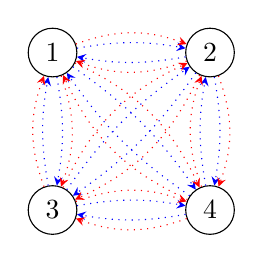
\begin{tikzpicture}
	\begin{scope}[every node/.style={circle,draw,align=center,text width = 5pt}]
		\node (1) at (0,0) {1};
		\node (2) at (2,0) {2};
		\node (3) at (0,-2) {3};
		\node (4) at (2,-2) {4};
	\end{scope}
	\begin{scope}[every edge/.style={dotted,draw,bend left=10},blue]
		\draw[-stealth] (1) edge (2);
		\draw[-stealth] (2) edge (1);
		\draw[-stealth] (1) edge (3);
		\draw[-stealth] (3) edge (1);
		\draw[-stealth] (1) edge (4);
		\draw[-stealth] (4) edge (1);
		\draw[-stealth] (2) edge (3);
		\draw[-stealth] (3) edge (2);
		\draw[-stealth] (2) edge (4);
		\draw[-stealth] (4) edge (2);
		\draw[-stealth] (3) edge (4);
		\draw[-stealth] (4) edge (3);
		
	\end{scope}
	\begin{scope}[every edge/.style={dotted,draw,bend left=20},red]
		\draw[-stealth] (1) edge (2);
		\draw[-stealth] (2) edge (1);
		\draw[-stealth] (1) edge (3);
		\draw[-stealth] (3) edge (1);
		\draw[-stealth] (1) edge (4);
		\draw[-stealth] (4) edge (1);
		\draw[-stealth] (2) edge (3);
		\draw[-stealth] (3) edge (2);
		\draw[-stealth] (2) edge (4);
		\draw[-stealth] (4) edge (2);
		\draw[-stealth] (3) edge (4);
		\draw[-stealth] (4) edge (3);
		
	\end{scope}
	\end{tikzpicture}
	\caption{Original network.\label{fig:problemexampleoriginal}}
	\end{subfigure}
	\vskip\baselineskip
	\begin{subfigure}[b]{0.45\textwidth}
	\hspace{-1cm}	
	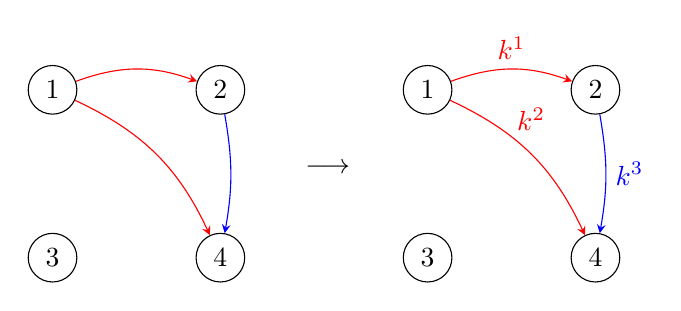
\begin{tikzpicture}
	\begin{scope}[every node/.style={circle,draw,align=center,text width = 5pt}]
		\node (1) at (0,0) {1};
		\node[right =1.5cm of 1] (2) {2};
		\node[below =1.5cm of 1] (3) {3};
		\node[right =1.5cm of 3] (4) {4};
		
		\node[draw=none] (arrow) at (3.3,-1) {$\longrightarrow$};		
		
		\node[right =2cm of 2] (1b) {1};
		\node[right =1.5cm of 1b] (2b) {2};
		\node[below =1.5cm of 1b] (3b) {3};
		\node[right =1.5cm of 3b] (4b) {4};
	\end{scope}
	\begin{scope}[every edge/.style={draw}]
		\draw[-stealth] (1) edge[red,bend left=20] node[above] {} (2);

		\draw[-stealth] (1) edge[red,bend left=20] node[above=5pt] {} (4);
		
		\draw[-stealth] (2) edge[blue,bend left=10] node[right] {} (4);

		\draw[-stealth] (1b) edge[red,bend left=20] node[above] {$k^1$} (2b);

		\draw[-stealth] (1b) edge[red,bend left=20] node[above=5pt] {$k^2$} (4b);
		
		\draw[-stealth] (2b) edge[blue,bend left=10] node[right] {$k^3$} (4b);
		
	\end{scope}
	\end{tikzpicture}
	\caption{Non-cooperative solution.\label{fig:problemexamplenotcoop}}
	\end{subfigure}
	\vskip\baselineskip
	\begin{subfigure}[b]{0.45\textwidth}
	\hspace{-1cm}	
	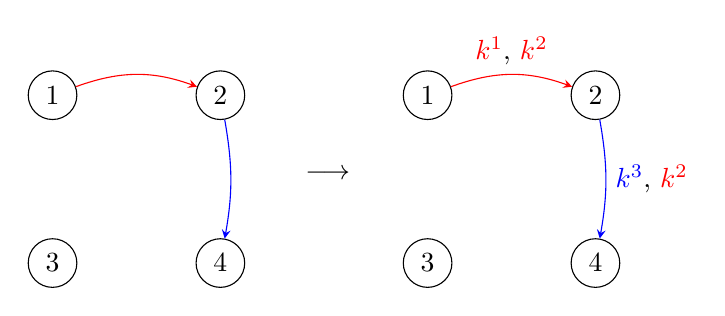
\begin{tikzpicture}
	\begin{scope}[every node/.style={circle,draw,align=center,text width = 5pt}]
		\node (1) at (0,0) {1};
		\node[right =1.5cm of 1] (2) {2};
		\node[below =1.5cm of 1] (3) {3};
		\node[right =1.5cm of 3] (4) {4};
		
		\node[draw=none] (arrow) at (3.3,-1) {$\longrightarrow$};				
		
		\node[right =2cm of 2] (1b) {1};
		\node[right =1.5cm of 1b] (2b) {2};
		\node[below =1.5cm of 1b] (3b) {3};
		\node[right =1.5cm of 3b] (4b) {4};
	\end{scope}
	\begin{scope}[every edge/.style={draw}]

		\draw[-stealth] (1) edge[red,bend left=20] node[above] {} (2);
		
		\draw[-stealth] (2) edge[blue,bend left=10] node[right] {} (4);
		
		\draw[-stealth] (1b) edge[red,bend left=20] node[above] {$k^1$\textcolor{black}{,} $k^2$} (2b);
		
		\draw[-stealth] (2b) edge[blue,bend left=10] node[right] {$k^3$\textcolor{black}{,} \textcolor{red}{$k^2$}} (4b);
	\end{scope}
	\end{tikzpicture}
	\caption{Cooperative solution.\label{fig:problemexamplecoop}}
	\end{subfigure}
	\caption{Example of a network design - multicommodity flow problem. \label{fig:problemexample}}
\end{figure}


On the rest of this section we introduce the specific characteristics of these problem as well as the notation we use during this work. We finish the section modelling the problem that each agent has to solve in case he does not take part of any collaboration alliance with other agents.

\subsection{Notation and detailed characteristics of the network design - multicomodity flow problem definition}
Let $N=\{1,...,n\}$ be the set of agents who form a coalition to cooperate. Let $G=(V,E)$ be a directed graph with
$V$ and $E$ its sets of nodes and edges respectively. 
Let $\Theta$ be the set of commodities the agents in the coalition have to serve. Each commodity $k$ has an origin node, $o(k)\in V$ and a destination node, $t(k)\in V$, and is owned by the agent $w(k)\in N$. Every commodity $k\in\Theta$ has a size of $d_k$ units and has an associated revenue $r_k$ per unit. Thus, the owner of the commodity $k$ earns a revenue of $d_k\cdot r_k$ if the commodity is successfully routed from its origin to its terminal node. The commodities are unsplitable, i.e., cannot be divided between different edges. Also, an agent do not necessary have to serve all his commodities.

For each edge $e \in E$, we note as $o(e)\in V$ its origin node and by $t(e)\in V$ its terminal node. Furtheremore, $w(e)\in N$ is the owner of the edge $e\in E$. Note that there can exist as many edges connecting a pair of nodes in an specific direction as agents in the coalition. Each edge $e \in E$ has certain units of capacity associated $q_e$, and a fixed activation
cost $c_e$. This activation cost is the price the owner of the edge has to pay if he wants to use the edge to route any commodity through it.

We will note by $\delta^+(v)\subset E$ the subset of edges whose origin is the node $v\in V$. Similarly, $\delta^-(v)\subset E$ is the subset of edges whose terminal node is $v\in V$. We will note by $E^i \subset E$ and $\Theta^i\subset \Theta$ the subsets of edges and commodities owned by agent $i$.

In table \ref{tb:notation} we summarize all the above introduced notation.

\begin{table}[ht!]
	\caption{Summary of notation. \label{tb:notation}}
	\begin{tabular}{|l|l|}
	\hline
	Symbol & Meaning	 \\ \hline
	$N$ & Set of agents. \\
	$G$ & Network. \\
	$V$ & Set of nodes in $G$. \\
	$E$ & Set of edges in $G$. \\
	$\Theta$ & Sets of commodities. \\
	$\delta^+(v)$ & Subset of edges in $E$ which depart from node $v$.\\
	$\delta^-(v)$ & Subset of edges in $E$ which arrive to node $v$.\\	
	$\Theta^i$ & Set of commodities owned by agent $i$. \\	
	$E^i$ & Set of edges owned by agent $i$.\\
	$E_A$ & Subset of edges in $E$ that are active. \\
	$E_R$ & Subset of edges in $E_A$ that have residual capacity.\\
	$k \in \Theta$ & A commodity.\\
	$o(k)$ & Origin node of commodity $k$.\\
	$t(k)$ & Destination node of commodity $k$.\\
	$w(k)$ & Agent who owns the commodity $k$.\\
	$d_k$ & Size, on units, of commodity $k$.\\
	$r_k$ & Revenue, per unit, associated with serving commodity $k$.\\
	$e\in E$ & An edge.\\
	$o(e)$ & Origin node of edge $e$.\\
	$t(e)$ & Terminal node of edge $e$.\\
	$w(e)$ & Agent who owns the edge $e$.\\
	$c_e$ & Cost of activate edge $e$. \\
	$q_e$ & Units of capacity of edge $e$. \\
	$q_e^R$ & Units of residual capacity of edge $e$.\\
	\hline
	\end{tabular}
\end{table}

\subsection{Single agent model}

The objective of an agent $i \in N$ is to maximize his payoff, routing his
commodities, $\Theta^i$, from their origin nodes to their terminal nodes through the edges he has activated,  $E_A^i\subset E^i$. We recall that an agent does not have to necessarily serve all his commodities. In any case, it would be easy to extend the models presented in this work to fulfil that condition. Also we assume that an agent has always the possibility of activate one, and only one, directed edge connecting two nodes $v$ and $w$ for any $v,w\in V$. In case we wanted to model a situation were some agents have not the possibility of activating certain edges, we could simply make the capacity of certain edges equal to 0, or make their activation cost a very big number, making the activation of that edges not profitable under any circumstance.

If an agent does not take part of the collaboration, he has not access to other agents' edges, neither the other agents can route their commodities through his edges. Thus, the problem which agent $i\in N$ has to solve when no cooperating with others can be modelled as the following ILP, that we call $P_i$,

    \begin{align}
        &  P_i: \quad \max  &  \sum_{k\in \Theta^i} \sum_{e \in \delta^+(t(k))\cap E^i} f_e^k \cdot d_k \cdot r_k - \sum_{e\in E^i} u_e\cdot c_e \hspace{20pt} &&   \label{eq:SingleAgentA}
    \end{align}
    \begin{align}
        & \text{subject to:}       &  \nonumber\\
       & \sum_{e \in \delta^-(z)\cap E^i} f_e^k-\sum_{e \in \delta^+(z)\cap E^i} f_e^k = 0,\quad && \forall\ z\in V\setminus\{o(k),t(k)\},\ \forall\ k\in\Theta^i,  \label{eq:SingleAgentB}\\
        &    \sum_{e \in \delta^+(t(k))\cap E^i} f_e^k \leq 1,  && \forall\ k\in \Theta^i, \label{eq:SingleAgentC} \\
		& \sum_{e \in \delta^+(t(k))\cap E^i} f_e^k= 0,  && \forall\ k\in \Theta^i, \label{eq:SingleAgentD} \\
		& \sum_{k \in \Theta^i} f_e^k \cdot d_k \leq u_e\cdot q_e, && \forall\ e \in E^i,\label{eq:SingleAgentE}  \\
		& \sum_{\substack{e \in E^i\colon \\ o(e),t(e) \in S}} f_e^k \leq |S| -1,   && \forall\ S \subset V,\ \forall\ k \in \Theta^i, \label{eq:SingleAgentF}\\[1em]
		& f_e^k \in \{0,1\},    && \forall\ e \in E^i,\ \forall\ k \in \Theta^i, \label{eq:SingleAgentG} \\ 
		&  u_e   \in \{0,1\},           && \forall\ e \in E^i,
    \end{align}

where, $\forall\ k\in \Theta^i$ and  $\forall\ e \in E$, $f_e^k$ and $u_e$ are decision variable such that
\[
\begin{array}{rl}
f_e^k = & \begin{cases}
    1 & \text{if commodity } k \text{ is routed through edge } e,\\
    0 & \text{otherwise}
\end{cases}  \\[20pt]
u_e = &\begin{cases}
    1 & \text{if edge } e \text{ is active},\\
    0 & \text{otherwise}    
\end{cases}
\end{array}
\]

The objective of agent $i$, equation (\ref{eq:SingleAgentA}), is to maximize the
profit generated by the commodities which arrive to their destination nodes
while minimizing the cost associated to the activation of the edges. Constraints
(\ref{eq:SingleAgentB}) ensure that, for any commodity, the flow that enters
and leaves every transit nodes (neither the origin, neither the terminal node of
that commodity) is equal. Constraints (\ref{eq:SingleAgentC}), together with
(\ref{eq:SingleAgentG}), guarantee that each commodity is send at most one time
from its origin node and that it is not split among different edges. Constraints (\ref{eq:SingleAgentD}) ensure that no
commodity is send from its terminal node to any other node. Constraints (\ref{eq:SingleAgentE})
ensure that the capacity of edges is not exceed. Finally, constraints
(\ref{eq:SingleAgentF}) are subtour elimination constraints \parencite{AHUJA1993}. 

%We have included it in our model because, first of all, it makes sense to assume that an agent would not want to create subtours when routing his commodities. Note that subtours could be possible without this constraint because once an edge is activated, there is no extra costs for routing more commodities through it. Furthermore, without the subtour elimination constraints, the other constraints are not sufficient to ensure that all the feasible solution of the ILP are admissible, since the flow of a commodity could contain a subtour disconneted from the origin and terminal nodes of that commodity, without impacting the objective but making the solution not valid for the problem we are modelling.

In a simplifying abuse of notation, we will refer with $P_i^*$ both to the value of the objective function for the optimal solution of $P_i$ as well as to the values that the decision variables have in that optimal solution. For instance, we can say that the edge $e\in E^i$ is active in the optimal solution of $P_i$ if $u_e=1$ in $P_i^*$. At the same time, we say that $P_i^*$ is the maximum payoff agent $i$ can obtain without collaborating with other agents. Furthermore, for any solution of $P_i$, if an edge $e\in E$ has been activated, we note by $q_e^R$ the residual capacity of that edge. We define the residual capacity of an active edge as the capacity which is still available in that edge after the routes of the commodities has been decided. If no commodities has been routed through an active edge $e$, then $q_e^R = q_e$. Furthermore, also for any solution of a network design - multicommodity flow problem. $E_A^i\subset E^i$ is the subset of active edges owned by the agent $i$, and $E_R^i\subset E_A^i$ the subset of active edges owned by agent $i$ with a positive residual capacity. 

\section{An allocation rule for a capacity exchange collaboration}
\label{seq:allocrule}
In all four different cooperation systems we present in this work, the members of a coalition can collaborate sharing at some price the capacity of the edges they have activated. This might allow some agents to serve commodities in a more efficient way with respect to the non-cooperative setting, and generate extra profit to the owners of the edges which are used by other agents.

In all the models presented in the next two sections, a proportional allocation rule is used to share the revenues and costs generated by the cooperation among the agents of the coalition. This proportional rule can be easily computed once a solution for the cooperative models is obtained, and it is characterized by the following conditions:
\begin{enumerate}
    \item The revenues generated by any served commodity are
    allocated to its owner.
    \item The activation cost of any active edge is paid by its owner.
    \item The price of using an unit of capacity on an edge $e\in E$ owned by agent $w(e)$ for any other member of the coalition, $i\in N\setminus\{w(e)\}$, is equal to $\dfrac{c_e}{q_e}$. Therefore,  if a commodity $k\in \Theta$ is routed through an edge $e	\in E$ and $w(k)\not = w(e)$, the agent who owns the commodity, $w(k)$ makes a side payment equal to $d_k \cdot\dfrac{c_e}{q_e}$ to the agent who owns the edge, $w(e)$.\footnote{The models could easily be adapted to allow the agents to individually choose the prices at which other agents can use capacity of their edges.}
\end{enumerate}

\section{Three cooperation systems with central authority} \label{seq:centrmodels}

In section \ref{seq:probdefinition} we have presented an ILP that models the network design -\\ multicommodity flow problem of an agent $i\in N$ who works alone. Now we present three different cooperative systems, where the agents in $N$ collaborate in different ways in order to find synergies among them and increase their payoffs.

The three models we propose in these section have in common the existence of a central authority which has some level of decision power. The first one, which we refer as the \emph{Fully centralized cooperation system} (FCCS) is a centralized planning system, where the central authority has full information and all the decision power. The other two models, the \emph{Partial cooperation system} (PCS) and the \emph{Residual cooperation system} (RCS), share a common structure composed of two stages which is based in the framework proposed in \textcite{ANUPINDI2001}. In the first stage, every agent $i\in N$ solves his individual problem without cooperating with the others, $P_i$, and shares with a central authority some information based in the optimal solution he has found (which information is exactly shared depends on the model). In the second stage, the central authority solves the cooperative problem, which is different in each of the two models, as it depends in the amount of information the agents has shared.

In table \ref{tb:summarycentralizedmodels} we summarize which decisions are left to the central authority and which are left to the agents in each model; and in table \ref{tb:summarycentralizedmodelsinfo} which information is shared by the agents. The Fully centralized cooperation systems (FCCS) assumes that full information is shared with the central authority, and all the decision power is given to him. In the Partial cooperation system (PCS), agents decide in the first stage which edges to activate and inform about their decisions as well as about all the commodities they have to serve to the central authority. Then, the central authority find the most efficient flow of all the commodities through the edges the agents have activated. Finally, in the Residual cooperation system (RCS), agents first decide which edges to activate and route their commodities through them, maximizing their individual payoffs. Then each agent shares with the central planner the commodities he has not served, which we note by $\Theta_R^i$, as well as his active edges which still have some residual capacity, $E_R^i$, together with how many units of exactly how many units of residual capacity each of that edges has. Then, in the second stage the central planner tries to route the residual commodities, $\Theta_R = \cup_i^n \Theta_R^i$ using the residual capacities of the residual edges, $E_R = \cup_i^n E_R^i$.

\begin{table}[ht!]
	\centering
	\caption{Summary of decision power allocation between agents and central authority. \label{tb:summarycentralizedmodels}}
    \begin{threeparttable}
        \begin{tabular}{p{0.1\textwidth}>{\centering}p{0.19\textwidth}>{\centering}p{0.15\textwidth}>{\centering}p{0.1\textwidth}>{\centering\arraybackslash}p{0.15\textwidth}}
            & &      \multicolumn{3}{c}{Coop. systems with central authority} \\\cline{3-5}
            & & FCCS &  PCS & RCS \\ \hline
            \multirow{2}{*}{Agents} & Activate edges & No & Yes & Yes \\
            & Route flow     & No & No & Yes \\\hline
            \multicolumn{1}{c}{Central} & Activate edges & Yes & No & No \\
 \multicolumn{1}{c}{Authority}          & Route flow & Yes & Yes & Yes\tnote{*} \\\bottomrule
        \end{tabular}
    \begin{tablenotes}\footnotesize
        \item[*] Only the residual commodities through the residual capacities
        of the active edges.
        \end{tablenotes}
    \end{threeparttable}
    \end {table}


\begin{table}[ht!]
	\centering
	\caption{Summary of the information the central authority has access to on each cooperative system with central authority. \label{tb:summarycentralizedmodelsinfo}}
\begin{tabular}{p{0.2\textwidth}p{0.1\textwidth}>{\centering}p{0.15\textwidth}>{\centering}p{0.15\textwidth}>{\centering\arraybackslash}p{0.15\textwidth}}
 & & \multicolumn{3}{c}{Coop. systems with central authority} \\\cline{3-5}
 & & FCCS & PCS & RCS \\\toprule
 \multirow{4}{*}{Commodities}  & $o(k),t(k)$ & $\forall\ k\in \Theta$ & $\forall\ k\in \Theta$  & $\forall\ k\in \Theta_R$  \\
 & $w(k)$    & " & " & " \\
 & $d_k$ & " & " & " \\
 & $r_k$ & " & " & " \\

\midrule
 \multirow{6}{*}{Edges}		 &  $o(e),t(e)$ & $\forall\ e\in E$ & $\forall\ e\in E_A$ & $\forall\ e\in E_R$\\
 			 & $w(e)$ & " & " & " \\
   			 & $c_e$  & " & " &  |\\
  			 & $q_e$  & " & " & |\\
 			 & $\frac{c_e}{q_e}$  & " & " &  $\forall\ e\in E_R$\\[3pt]
 			 & $q_e^R$  & | & | & " \\\bottomrule

\end{tabular}


\end{table}

In the rest of this section we present in a more detailed way the three different
cooperative systems with central authority with decision power we propose in this work.


\subsection{Fully centralized cooperation system (FCCS)}

We start introducing the model where more power is given to the central planner.
In the Fully centralized cooperation system (FCCS), the agents share all their commodities' and edges' information with the central authority. Each agent also inform to the central planner about which is the maximum payoff they can obtain without cooperating (this is something that can be computed by the agents, or by the central planner itself since it has all the required information to do it). Then, the central authority solves a new ILP, $\Gamma_F$, which is almost identical to $P_ i$, the ILP that an agent $i\in N$ has to solve when no cooperating. Both problems only differ in
two aspects (see Appendix \ref{seq:appendixilpfull} for a complete overview of the ILP):

\begin{enumerate}
	\item The central planner manages all the commodities and edges of all the agents, $\Theta$ and $E$, while without cooperation an agent $i$ only has access to his own commodities and edges, $\Theta^i$ and $E^i$.
	\item The following two new constraints are added to the problem:

\begin{equation}
\sum_{e \in \delta^-(t(k))}  f_e^k \cdot d_k \cdot r_k - \sum_{\substack{e \in E^j\colon \\ j\not = i}} f_e^k \cdot d_k \cdot \frac{c_e}{q_e}\geq 0,  \forall\ k \in \Theta, \label{eq:commodirevenue}
\end{equation}
\begin{equation}
\varphi_i(\Gamma_F) \geq P_i^*,  \forall\ i\in N; \label{eq:newconstraintFullCooperation}
\end{equation}

Constraints (\ref{eq:commodirevenue}) avoids that the central planner serves a commodity in such a way that the side payments his owner has to make are higher than the revenue he obtains for serving that commodity. Furtheremore, with constraints (\ref{eq:newconstraintFullCooperation}), similarly to the idea introduced by \textcite{VANOVERMEIRE2014125}, we integrate the final payoffs of the agents, $\varphi_i(\Gamma_F)$ for each $i \in N$, in the constraints of the central planner's problem. Thus, these constraints  ensure that the final payoff of every agent is greater or equal than what that agent could achieve without cooperation, i.e., $P_i^*$.  Doing so we ensure that the final payoff allocation is \emph{individually rational} \parencite{GONZALEZ2010}, i.e., no single agent is interested in leaving the coalition unilaterally.  \footnote{We can extend this idea by forcing the solution resulting from the cooperation to be in the \emph{core}, by adding constraints ensuring that the sum of the payoffs of the members of any subcoalition of $N$ is greater than what that agents could obtain by leaving the grand coalition and cooperating only among them. Nevertheless, doing it will increase the complexity of the models and we consider that it does not add value to this work.}

For each agent $i\in N$, we define its final payoff in the FCCS $\varphi_i(\Gamma_F)$ as

\begin{equation}
    \hspace{-10pt}\begin{split}
    & \varphi_i(\Gamma_F) =\label{eq:FullCooperationPayoff} \\
    & = \sum_{(o,t,i)\in \Theta^i} \left[ \sum_{e \in \delta^-(t)\cap E^i} f_e^{(o,t,i)} \cdot d_{(o,t,i)} \cdot r_{(o,t,i)} -  \sum_{\substack{e\in \Theta^j \colon\\ j\not = i}} f_e^{(o,t,i)} \cdot d_{(o,t,i)} \cdot \frac{c_e}{q_e} \right]  \\
    & + \sum_{\substack{(o,t,k) \in \Theta  \colon \\ k \not = i}} \left[\sum_{e \in E^i} f_e^{(o,t,k)} \cdot d_{(o,t,k)} \cdot \frac{c_e}{q_e}\right] - \sum_{e \in E^i} u_e \cdot c_e, 
    \end{split}
\end{equation}

\end{enumerate}


The first term of equation (\ref{eq:FullCooperationPayoff}) is the sum of the profit associated with the commodities of the agent, which for each commodity is equal to the revenue it
generates when it is served minus the cost the agent has to pay to other agents if the commodity passes through edges which does not belong to him. The second sum is the payments that other agents make to him when routing their commodities through his edges. The last term is the sum of the costs of the active edges which belong to the agent.

\subsection{Partial cooperation system (PCS)}

In the Partial cooperation system (PCS), the central authority has to optimize once again the flow of all the commodities of all the agents through the network, maximizing the total generated revenue. Nevertheless, the decision of which edges to activate remains as an individual decision of each agent.


\begin{figure}[ht!]
\centering
\caption{Flowchart of the Partial cooperation system. \label{fig:partialmodel}}
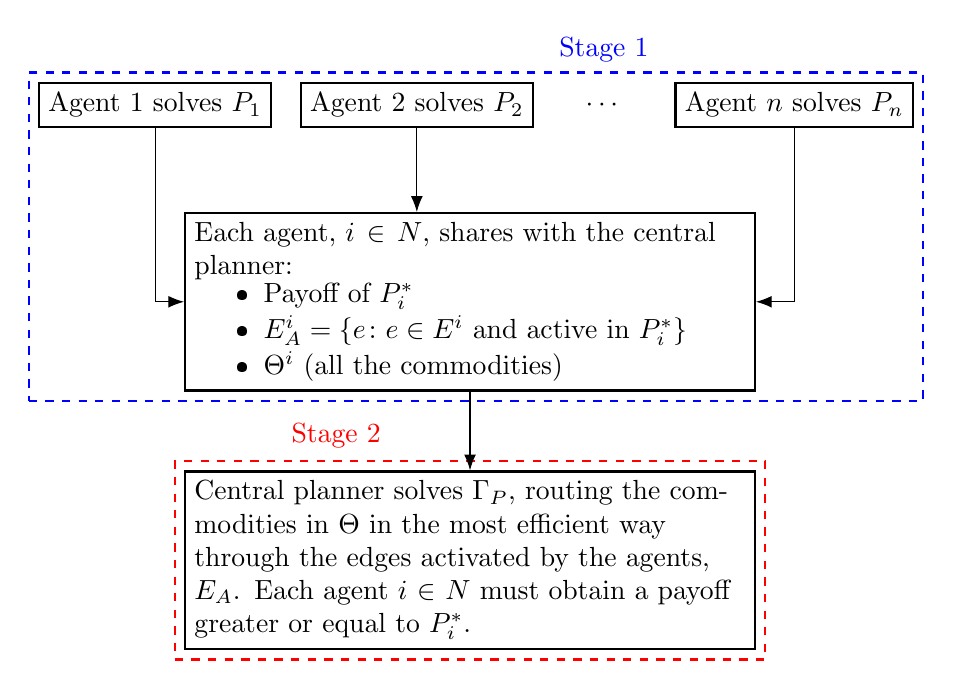
\begin{tikzpicture}
	\begin{scope}[every node/.style={rectangle,draw,thick,minimum height=16pt,minimum width =30pt}]
		\node (A1) at (-4,0) {Agent 1 solves $P_1$};
		\node[right =10pt of A1] (A2) {Agent 2 solves $P_2$};
		\node[draw=none,right =10pt of A2] (pass) {$\cdots$ };
		\node[right =10pt of pass] (An) {Agent $n$ solves $P_n$};
		\node[align = left,text width=7cm] (shares) at (0,-2.5) {Each agent, $i\in N$,  shares with  the  central planner:\vspace{-10pt}
		\begin{itemize}
			\itemsep-3pt 
        		\item Payoff of $P_i^*$
        		\item $E_A^i=\{e\colon e\in E^i \text{ and active in } P_i^*\}$
        		\item $\Theta^i$ (all the commodities)
   		 \end{itemize}
    };
    \node[below = of shares,align = left,text width=7cm] (central) {Central planner solves $\Gamma_P$, routing the commodities in $\Theta$ in the most efficient way through the edges activated by the agents, $E_A$. Each agent $i\in N$ must obtain a payoff greater or equal to $P_i^*$.};
    
    \node [fit=(A1) (An) (shares),draw,dashed,thick,blue] {};
    \node[draw=none,blue] (Stage1) at (1.7,0.7) {Stage 1}	;
 	\node [fit=(central) ,draw,dashed,thick,red] {};
 	\node[draw=none,red] (Stage2) at (-1.7,-4.2) {Stage 2}	;
	
	\end{scope}
	
	\begin{scope}
	\draw[-{Latex[length=2mm]}] (A1.south) |- (shares.west);
	\draw[-{Latex[length=2mm]}] (A2) edge (A2.south|-shares.north);
	\draw[-{Latex[length=2mm]}] (An.south) |- (shares.east);
	\draw[-{Latex[length=2mm]}] (shares) edge (central);

	\end{scope}
\end{tikzpicture}
\end{figure}

In a first stage, every agent $i \in N$ solves his own $P_i$ problem. Then, each agent $i\in N$ shares with the central authority all his commodities, $\Theta^i$, and inform about which is the maximum payoff he can obtain without cooperating, $P_ i^*$ and which edges he would activate in that case, $E_A^i=\{e\colon u_e=1 \text{ in } P_i^*\}$. In the second stage, the central authority solves a new ILP, $\Gamma_P$, routing all the commodities of all the agents, $\Theta=\cup_{i=1}^n \Theta^i$, through all the edges agents would have activated in the non-cooperation scenario, $E_A=\cup_{i=1}^n E_A^i$, maximizing the profit of the total coalition while ensuring no agent $i\in N$ get a payoff lower than $P_i^*$. In figure \ref{fig:partialmodel} we present a flowchart summarizing these steps.

The ILP, $\Gamma_P$, corresponding to the cooperative problem that the central planner has to solve in the PCS is

\begin{align}
        &  \Gamma_P: \max  & \sum_{k \in \Theta} \sum_{e \in \delta^-(t(k))\cap E_A}  f_e^k \cdot d_k \cdot r_k  &&   \label{eq:PartialCooperationA} 
    \end{align}
    \begin{align}
        & \text{subject to:}       && \nonumber\\
        & \sum_{e \in \delta^-(z)\cap E_A} f_e^k-\sum_{e \in \delta^+(z)\cap E_A} f_{e}^k = 0,            \quad && \forall\ z\in V\setminus\{o(k),t(k)\},\nonumber\\
& && \forall\ k\in\Theta,  \label{eq:PartialCooperationB}\\[1em]
& \sum_{e \in \delta^+(o(k))\cap E_A} f_e^k \leq 1,  && \forall\ k\in \Theta, \label{eq:PartialCooperationC} \\
& \sum_{e \in \delta^+(t(k))\cap E_A} f_e^k = 0,  && \forall\ k\in \Theta, \label{eq:PartialCooperationD} \\
 & \sum_{k \in \Theta} f_e^k\cdot d_k \leq q_e     && \forall\ e \in E_A, \label{eq:PartialCooperationE}  \\
 & \sum_{\substack{e \in E_A\colon \\ o(e),t(e) \in S}} f_e^k  \leq |S| -1,    && \forall\ S \subset V,\ \forall\ k \in \Theta, \label{eq:PartialCooperationF}\\
&\sum_{e \in \delta^-(t(k))\cap E_A}  f_e^k \cdot d_k \cdot r_kk
 -\sum_{\substack{e \in E_A^j\colon \\ j\not = i}} f_e^k \cdot d_k \cdot \frac{c_e}{q_e}\geq 0, && \forall\ k \in \Theta, \label{eq:PartialCooperationG} \\
& \varphi_i(\Gamma_P)   \geq P_i^*,     && \forall\ i\in N \label{eq:PartialCooperationH}\\
 & f_e^k  \in \{0,1\},    && \forall\ e \in E_A, \forall\ k \in \Theta, \label{eq:PartialCooperationI}
    \end{align}

Note that, this model differs from the previously presented in this work in the absence of decisions variables for the activation of the edges, since this decision is previously made by the agents and not left to the central planner. Also, we include the constraints (\ref{eq:PartialCooperationG}) and (\ref{eq:PartialCooperationH})
which are equivalent to the constraints (\ref{eq:commodirevenue}) and (\ref{eq:newconstraintFullCooperation}) in FCCS. In this case, because the absence of the decision variables $u_e$ in the model, we redefine the payoffs allocate to each agent $i\in N$ as follows:

\begin{equation}
    \begin{split}
    & \varphi_i(\Gamma_P) =\label{eq:PartialCooperationPayoff} \\
    & = \sum_{k\in \Theta^i} \left[ \sum_{e \in \delta^-(t(k))\cap E_A} f_e^k \cdot d_k \cdot r_k -  \sum_{\substack{e\in E_A \colon\\ w(e)\not = i}} f_e^k \cdot d_k \cdot \frac{c_e}{q_e} \right] + \\
    & + \sum_{\substack{k \in \Theta  \colon \\ t(k) \not = i}} \left[\sum_{e \in E_A^i} f_e^k \cdot d_k \cdot \frac{c_e}{q_e}\right] - \sum_{e \in E_A^i} c_e.
    \end{split}
\end{equation}

\subsection{Residual cooperation system (RCS)}

In the Residual cooperation system (RCS), the agents once again start by solving in the first stage their individual problems, $P_i$ for each $i\in N$. Nevertheless, this time the agents  would actually implement the optimal solution they found for those problems, $P_i^*$ for each $i\in N$. Then, they would inform the central authority about which commodities they were not able to serve when working alone, $\Theta_R^i$, as well as which edges they have activated still have some residual capacity $E_R^i$. In the second stage, the central authority routes the residual commodities of all the agents $\Theta_R = \cup_{i=1}^n \Theta_R^i$ through the edges with residual capacity, $E_R=\cup_{i=1}^n E_R^i$. Furtheremore, the sum of the sizes of the commodities the central authority routes through an edge $e\in E_R$ cannot exceed the residual capacity of that edge, which we note by $q_e^R$. That residual capacity is equal to the capacity that the owner of that edge, $w(e)\in N$, has not used after implementing $P_{w(e)}^*$.
Figure \ref{fig:residualmodel} shows an overview of the structure of this system.


\begin{figure}[ht!]
\centering
\caption{Flowchart of the Residual cooperation system. \label{fig:residualmodel}}
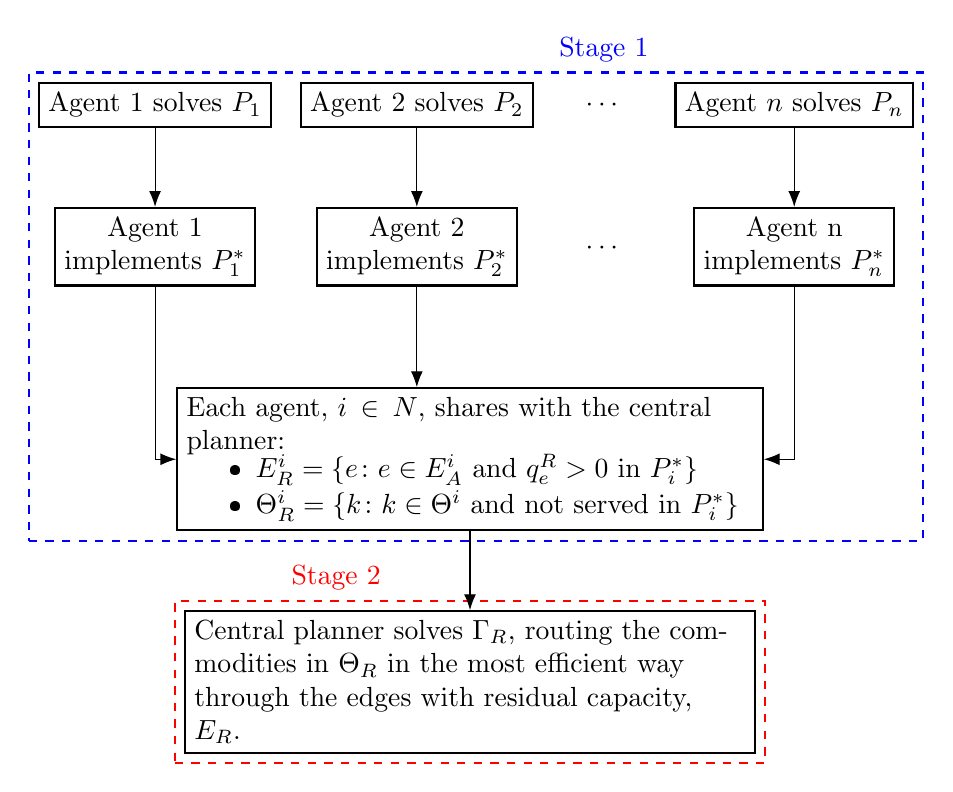
\begin{tikzpicture}
	\begin{scope}[every node/.style={rectangle,draw,thick,minimum height=16pt,minimum width =30pt}]
		\node (A1) at (-4,0) {Agent 1 solves $P_1$};
		\node[right =10pt of A1] (A2) {Agent 2 solves $P_2$};
		\node[draw=none,right =10pt of A2] (pass) {$\cdots$ };
		\node[right =10pt of pass] (An) {Agent $n$ solves $P_n$};
		\node[below = of A1,align = center] (A1impl) {Agent 1 \\ implements $P_1^*$};
		\node[below = of A2,align = center] (A2impl) {Agent 2 \\ implements $P_2^*$};
		\node[draw=none,below =35pt of pass] (pass2) {$\cdots$ };
		\node[below = of An,align = center] (Animpl) {Agent n \\ implements $P_n^*$};
		\node[align = left,text width=7.2cm] (shares) at (0,-4.5){Each agent, $i\in N$,  shares with  the  central planner:\vspace{-10pt}
		\begin{itemize}
			\itemsep-3pt
        		\item $E_R^i=\{e\colon e\in E_A^i \text{ and } q_e^R>0 \text{ in } P_i^*\}$
        		\item $\Theta_R^i=\{k\colon k\in\Theta^i\text{ and not served in } P_i^*\}$
   		 \end{itemize}
    };
    \node[below = of shares,align = left,text width=7cm] (central) {Central planner solves $\Gamma_R$, routing the commodities in $\Theta_R$ in the most efficient way through the edges with residual capacity, $E_R$.};
    
	  \node [fit=(A1) (An) (shares),draw,dashed,thick,blue] {};
    \node[draw=none,blue] (Stage1) at (1.7,0.7) {Stage 1}	;
 	\node [fit=(central) ,draw,dashed,thick,red] {};
 	\node[draw=none,red] (Stage2) at (-1.7,-6) {Stage 2}	;    
    
	\end{scope}
	
	\begin{scope}
	\draw[-{Latex[length=2mm]}] (A1) edge (A1impl);
	\draw[-{Latex[length=2mm]}] (A2) edge (A2impl);
	\draw[-{Latex[length=2mm]}] (An) edge (Animpl);
	\draw[-{Latex[length=2mm]}] (A1impl.south) |- (shares.west);
	\draw[-{Latex[length=2mm]}] (A2impl) edge (A2.south|-shares.north);
	\draw[-{Latex[length=2mm]}] (Animpl.south) |- (shares.east);
	\draw[-{Latex[length=2mm]}] (shares) edge (central);

	\end{scope}
\end{tikzpicture}
\end{figure}

The ILP the central planner has to solve in the residuals cooperation system, $\Gamma_R$, is equivalent to $\Gamma_P$, but the commodities and edges the central planner manages are $\Theta_R$ and $E_R$ instead of $\Theta$ and $E_A$. Also, as the central planner cannot route commodities through an edge $e\in E_R$ exceeding the residual capacity of that edge, $q_e^R$, the constraints (\ref{eq:PartialCooperationE}) are substituted by

\begin{equation}
\sum_{k \in \Theta_R} f_e^k\cdot d_k \leq q_e^R,\quad \forall\ e \in E_R.
\end{equation}
in the model of this cooperative problem (see Appendix \ref{seq:appendixilpresidual} for a full overview of the ILP).
    
In this system, it is guaranteed by design that each agent receives  payoff greater or equal than the payoff they could obtain by their own, as they always first implement the best solution they can achieve without cooperating. Therefore they can only increase their payoffs with respect to that value and constraints equivalent to (\ref{eq:PartialCooperationH}) are not required. Under the Residual cooperation system we define the final payoff of an agent $i\in N$ as

\begin{equation}
    \begin{split}
    & \varphi_i(\Gamma_R) =\label{eq:ResidualCooperationPayoff} \\
    & = \sum_{k\in \Theta^i_R} \left[ \sum_{e \in \delta^-(t(k))\cap E_R} f_e^k \cdot d_k \cdot r_k -  \sum_{\substack{e\in E_R \colon\\ w(e)\not = i}} f_e^k \cdot d_k \cdot \frac{c_e}{q_e} \right] + \\
    & + \sum_{\substack{k \in \Theta_R  \colon \\ w(k) \not = i}} \left[\sum_{e \in E_R^i} f_e^k \cdot d_k \cdot \frac{c_e}{q_e}\right] + P_i^*
    \end{split}
\end{equation}


\section{An fully decentralized iterative cooperation system for two agents} \label{seq:itermodel}

In this section we propose a fully decentralized iterative cooperation system (FDICS) for two agents, where all the decisions are left to the members of the coalition, and therefore there is not any central authority, but the members of the coalition make use of an \emph{information platform} to interact with each other.

The idea behind this mechanism is that the agents exchange information in an iterative process, informing to the other agent about the residual capacity they have in their own active edges, allowing him to use that residual capacity to route his commodities at some price.

Before going in more detail about the cooperation mechanism structure, we introduce how the information platform works. Each agent $i\in N$ has two different ``pools" to share information:

\begin{description}
	\item[Shared edges:] Agent $i$ can share a subset of his active edges which still have some residual capacity, $\widehat{E}_R^i\subseteq E_R^i$. He also has to share how many units of residual capacity has each edge $e\in \widehat{E}_R^i$, $q_e^R$, and at which price the other agent can use each of that units, $\frac{c_e}{q_e}$
	\item[Demanded edges:] If agent $j\in N$ has previously shared a set of edges in the platform, agent $i\in N\setminus\{j\}$ can use those edges when routing his commodities. If agent $i$ actually decides to route a subset of his commodities, $\widehat{\Theta}^i\subset \Theta ^i$ through some of that edges, he has to share in the information platform:
	\begin{enumerate}
		\item How much units of capacity he requires (or demands) in total on each edge $e$ shared by agent $j$, what we note by $q_e^D$.
	\item For each commodity $k\in \widehat{\Theta}^i$, a set $L^k$, containing the edges shared by agent $j$ through which the commodity $k$ would be routed. Note that a commodity $k\in \widehat{\Theta}^i$ might be routed through edges owned by agent $i$ and/or trough edges shared by agent $j$. The latter are the ones which must be included in $L^k$. Also he has to share which is the size of that commodity, $d_k$, allowing agent $j$ to know which would be the side payment, $p_k$, he would receive if finally all the edges $e$ in $L^k$ are active and he can make use of $q_e^D$ units of capacity in each of them\footnote{\label{ft:sidepaymentexplanation}
Note that the condition agent $j$ has to accomplish in order to receive the side payment associated with a commodity $k\in\widehat{\Theta}^i$, $p_k$, is to left available the total capacity agent $i$ has demanded in each $e\in L^k$, $q_e^D$, even if it is possible that $q_e^D\geq d_k$ for some $e\in L ^k$, as agent $i$ might be willing to route several commodities through that edge.}.
That side payment associated to the commodity $k\in \Theta^i$ is computed as $p_k=\sum_{e \in L^k} d_k\cdot \frac{c_e}{q_e}$. 
	\end{enumerate}
		
\end{description}	

Making use of the information platform just introduced, both agents iteratively solve an ILP. In each iteration both agents sequentially (one after the other and not at the same time) decide which edges to activate, and how to route their commodities through the network, as they do in $P_i$. Nevertheless, in this cooperation system they can also route their commodities through the edges shared in the platform by the other agent with the corresponding costs and respecting the available capacities on that edges. Furthermore, when deciding if an edge should be activated or not, each agent does not only have to account for the activation cost, but also for the side payments the other agent is willing to make to him if he activates certain combinations of edges and leaves on them certain units of capacity available to the other agent. The ILP, $\Upsilon_i$, agent $i\in N$ has to solve in each iteration is the following:

    \begin{align}
        &  \Upsilon_i: \hspace{10pt} \max  &&  \sum_{k\in \Theta^i} \sum_{e \in \delta^-(t(k))\cap (E^i\cup \widehat{E}_R^j)} f_e^k \cdot d_k \cdot r_k - \sum_{e\in E^i} u_e\cdot c_e \hspace{20pt} -  \nonumber  \label{eq:IterativeA}\\
        & 								  && - \sum_{k \in \Theta^i} \sum_{\substack{e \in \widehat{E}_R^j\colon \\ j\not = i}} f_e^k \cdot d_k \cdot \frac{c_e}{q_e}   + \sum_{\substack{k \in \widehat{\Theta}^j \colon \\j\not = i}} p_k \cdot t_k
    \end{align}
    \begin{align}
        & \text{subject to:}       && \nonumber\\
& \sum_{e \in \delta^-(z)\cap (E^i\cup \widehat{E}_R^j)} f_e^k-\sum_{e \in \delta^+(z)\cap (E^i\cup \widehat{E}_R^j)} f_{e}^k  = 0,                                   && \forall\ z\in V\setminus\{o(k),t(k)\},\nonumber\\[-1em]
& && \forall\ k\in\Theta^i,  \label{eq:IterativeB}\\[1em]
& \sum_{e \in \delta^+(o(k))\cap (E^i\cup \widehat{E}_R^j)} f_e^k  \leq 1, && \forall\ k\in \Theta^i, \label{eq:IterativeC} \\
& \sum_{e \in \delta^+(t(k))\cap (E^i\cup \widehat{E}_R^j)} f_e^k  = 0,  && \forall\ k\in \Theta^i, \label{eq:IterativeD} \\
& \sum_{k \in \Theta^i} f_e^k\cdot d_k \leq u_e\cdot q_e, && \forall\ e \in E^i, \label{eq:IterativeE}  \\
& \sum_{k \in \Theta^i} f_e^k\cdot d_k \leq  q_e^R, && \forall\ e \in \widehat{E}_R^j,\label{eq:IterativeF}  \\
& \sum_{\substack{e \in E^i\cup \widehat{E}_R^j\colon \\ o(e),t(e) \in S}}  f_e^k  \leq |S| -1, && \forall\ S \subset V,\ \forall\ k \in \Theta^i, \label{eq:IterativeG}\\
&\sum_{k\in \Theta^i} f_e^k \cdot d_k \leq (q_e - q_e^D) +M(1-b_e),\quad && \forall e \in \bigcup_{\bar{k} \in \widehat{\Theta}^j}L^{\bar{k}}, \label{eq:IterativeH}\\
&b_e \leq u_e, && \forall e\in \bigcup_{k \in \widehat{\Theta}^j}L^k, \label{eq:IterativeI}\\
& t_k \leq 1 -  (|L^k|-\sum_{e \in L^k} b_e), && \forall k \in \widehat{\Theta}^j \label{eq:IterativeJ}\\
& f_e^k  \in \{0,1\}, && \forall\ e \in E^i,\ \forall\ k \in \Theta^i, \label{eq:IterativeK} \\
&  u_e   \in \{0,1\},   && \forall\ e \in E^i,  \label{eq:IterativeL}\\
& b_e \in \{0,1\}, && \forall e \in \bigcup_{k\in \widehat{\Theta}^j}L^k,\label{eq:IterativeM}\\
& t_k \in \{0,1\}, && k \in \widehat{\Theta}^j, \label{eq:IterativeN}
    \end{align}
where $M$ is a very large value  and $\forall\ e \in \cup_{k\in\widehat{\Theta}^j}L^k$ and $\forall\ k\in \widehat{\Theta}^j$, $b_e$ and $t_k$ are decision variables such that
\[
\begin{array}{rl}
b_e = & \begin{cases}
    1 & \text{if edge } e \text{ is active and its residual capacity, } q_e^R\text{, is not greater} \\[-2pt]
    & \text{than the total capacity demanded by the other agent, } q_e^D,\\
    0 & \text{otherwise;}
\end{cases}  \\[20pt]
t_k = &\begin{cases}
    1 & \text{if } \forall e \in L^k \text{ the conditions to receive the side payment } p_k \text{ are} \\[-2pt]
    & \text{fulfilled},\\
    0 & \text{otherwise.}    
\end{cases}
\end{array}
\]

In $\Upsilon_i$, the first term of the objective function of the agent $i$, equation (\ref{eq:IterativeA}), is the sum of the revenue generated by the commodities which are served. The second term is the sum of the costs of the edges he has activate. The third term is the sum of the side payments he has to do when routing commodities through the edges shared by the other agent. Finally, the fourth term is the sum of the side payments he receives from the other agent for making use of the edges he has shared in the previous iteration, if they remain available in the conditions the other agent has demanded.

Constraints (\ref{eq:IterativeB}), (\ref{eq:IterativeC}), (\ref{eq:IterativeD}) and (\ref{eq:IterativeG}) are equivalent to constraints (\ref{eq:SingleAgentB}),(\ref{eq:SingleAgentC}),(\ref{eq:SingleAgentD}) and (\ref{eq:SingleAgentF}) in $P_i$, with the difference that now the agent $i$ can use the edges shared in the information platform by the agent $j$, $\widehat{E}_R^j$. Constraints (\ref{eq:IterativeE}) are identical to constraints (\ref{eq:SingleAgentE}) and constraints (\ref{eq:IterativeF}) are an extension of them, ensuring that the agent does not exceed the residual capacity of the edges shared by agent $j$ when routing his commodities.

Constraints (\ref{eq:IterativeH}),  (\ref{eq:IterativeI}) and (\ref{eq:IterativeJ}) together with the decision variables (\ref{eq:IterativeM}) and (\ref{eq:IterativeN}), are related with the side payments agent $i$ receives from agent $j$. Recall for each commodity $k\in \widehat{\Theta}^j$, $L^k$ is the set which contains the edges of agent $i$ that agent $j$ has indicated in the previous iteration he would like to use to route commodity $k$. Note agent $j$ could be interested in routing multiple commodities through the same edge $e$ of agent $i$, therefore $e$ could be an element of multiple sets $L^k$. He has also indicates how many units of capacity in total, $q_e^D$ he requires in each edge $e\in \cup_{k\in\widehat{\Theta}^j}L^k$. If and only if in each edge $e \in L^k$, all the units of capacity  he has demanded are available, he would route the commodity $k$ using that edges, and consequently make the associated side payment, $p_k$, to agent $i$. Constraints (\ref{eq:IterativeJ}) and (\ref{eq:IterativeN}) ensure that $t_k$ can only be equal to 1 if all the decision variables $b_e$ for $e \in L^k$ are also equal to 1. At the same time, constraints (\ref{eq:IterativeH}),  making use of the \emph{big M} coefficient, and (\ref{eq:IterativeI}) ensures that if $b_e$ is equal to 1, indeed agent $i$ leaves at least $q_e^D$ units of residual capacity on edge $e$ and activates it. Note that these constraints are actually too restrictive: as already introduced in the footnote of page \pageref{ft:sidepaymentexplanation}, agent $j$ might be planning to route 2 or more commodities through the edge $e$, and even if agent $i$ leaves less units of capacity available than the demanded ones, $q_e^D$, he might be able to route, not all, but some of that commodities through it. However, these constraints assume that none of the commodities could be routed and therefore, ensuring that  agent $i$ does not expect to receive any side payment associated with the commodities agent $j$ wanted to route through that edge. We argue that capture with accuracy a more realistic behaviour, computing which commodities could still be routed through an edge with a residual capacity available smaller than the total demanded capacity by the other agent would make the model too complex. Indeed if agent $i$ decides to leave less available capacity in an edge, $q_e^R$, than the total capacity demanded by agent $j$, $q_e^D$, the problem of deciding which commodities to include in the route is a \emph{knapsack problem}, which has been proven to be NP-complete \parencite{KARP1972}.

In figure \ref{fig:iterflowchart} we present a flow chart illustrating the global structure of these cooperation mechanism.
In each iteration and in order, after solving $\Upsilon^1$ or $\Upsilon^2$ respectively, agents update the information they share in the information platform. The iterative process continues until an equilibrium is found or a fixed maximum number of iterations allowed is reached. We define an \emph{equilibrium} as the situation were the solutions of $\Upsilon^1$ and $\Upsilon^2$ found in the iteration $h$ are exactly the same than the solutions found in the iteration $h-1$. This is equivalent to the definition of the \emph{Nash equilibrum}: given the strategies of all the agents, an agent cannot individually improve their payoffs by changing his own strategy \parencite{GONZALEZ2010}. If no equilibrium is reached in the maximum number of iterations allowed, the system considers that no solution for the cooperation was found. Note that in the first iteration, as the information platform is empty, agent 1 is in practice solving $P^1$. Indeed, at any moment if no information was shared in the platform, $\Upsilon^i=P^i$. For the same reason, in the first iteration agent 2 does not expect any side payments from agent 1, since he have not got yet the opportunity of demanding any edges, as no edges were shared by agent 2 in the platform when agent 1 solved $\Upsilon^1$ in the first iteration. 


\begin{figure}[ht!]
\centering
\caption{Flowchart of the decentralized cooperation mechanism for two agents.\label{fig:iterflowchart}}
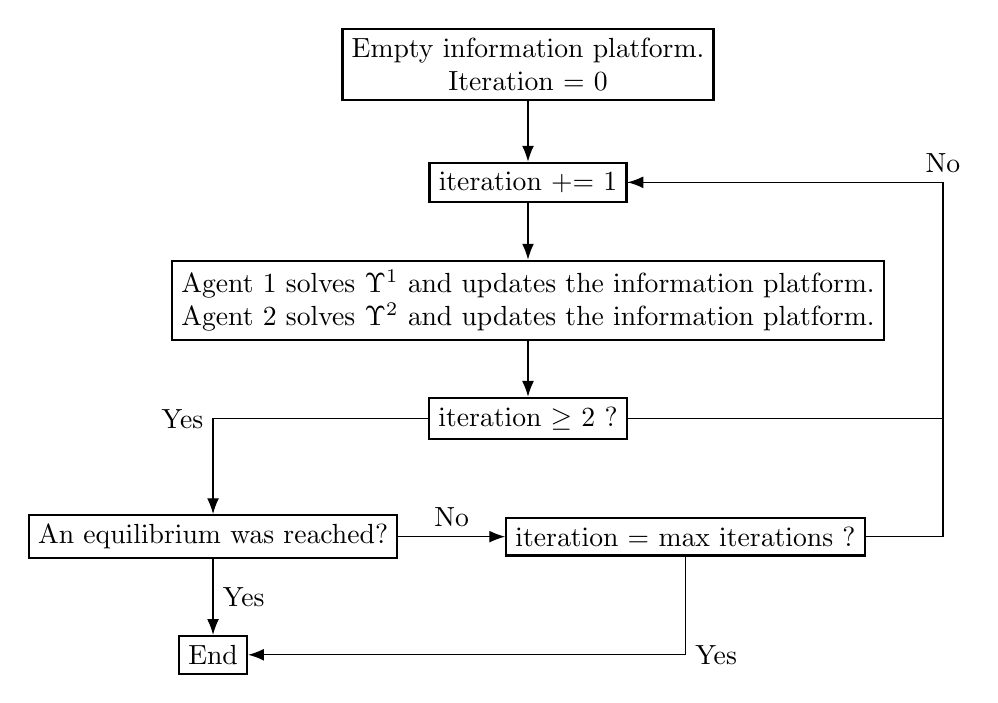
\begin{tikzpicture}
\begin{scope}[every node/.style={rectangle,draw,thick}]
	\node[align = center] (init) at (0,0)  {Empty information platform.\\
	Iteration = 0};
	\node (iteration) at (0,-1.5){iteration += 1};
	\node[align =left] (main) at (0,-3) {Agent 1 solves $\Upsilon^1$  and updates the information platform.\\
	Agent 2 solves $\Upsilon^2$  and updates the information platform.};
	\node (itquestion) at (0,-4.5) {iteration $\geq$ 2 ?};

	\node (equiquestion) at (-4,-6) {An equilibrium was reached?};

	\node (maxit) at (2,-6) {iteration = max iterations ?};

	\node (End) at (-4,-7.5) {End};
\end{scope}

\begin{scope}
	\draw[-{Latex[length=2mm]}] (init) edge (iteration);
	\draw[-{Latex[length=2mm]}] (iteration) edge (main);
	\draw[-{Latex[length=2mm]}] (main) edge (itquestion);
	\draw[-{Latex[length=2mm]}] (itquestion.east)  -- ++(4cm,0) |- node[above] {No}
	 (iteration.east);
	\draw[-{Latex[length=2mm]}] (itquestion.west) -| node[left] {Yes} (equiquestion);
	\draw[-{Latex[length=2mm]}] (equiquestion)  edge node[above] {No} (maxit);
	\draw[-{Latex[length=2mm]}] (equiquestion) edge node[right] {Yes} (End);
	\draw[-{Latex[length=2mm]}] (maxit.south) |- node[right] {Yes} (End);
	\draw[-] (maxit.east)  -- ++(0.98cm,0) |- (iteration.east);
\end{scope}
\end{tikzpicture}
\end{figure}

We finish this section highlighting the differences in terms of information sharing and decision power allocation between this Fully decentralized iterative cooperation system (FDICS) and the others mechanism presented in section \ref{seq:centrmodels}. First of all, we recall that in the FDICS all the decisions are left to the agents, and the central authority with decision power present in the FCCS, the PCS and the RCS is substituted by an information platform. In the other side, the amount of information agents share in that information platform in the FDICS is also smaller than what the agents share with the central authority in any of the first three systems. In FDICS, an agent $i\in N$ does not have to make public in any moment information about his commodities, with the exception of the size, $d_k$, for the commodities $k\in \Theta^i$ he wants to route through edges of the other agent $j\in N\setminus\{i\}$. This means that the revenues associated to each commodity, as well as its origin and destination nodes remain private information during the whole cooperation process. However, the information an agent shares with the information platform in the FDICS relative to his edges is equivalent to the information an agent shares with the central authority in the Residual cooperation system (RCS) (recall table \ref{tb:summarycentralizedmodelsinfo}).

\section{Results} \label{seq:results}

In order to analyse the performance of the different models discussed in this work, we tested the 4 different cooperation systems over 20 instances of the network design - multicommodity flow problem introduced in section \ref{seq:probdefinition}. We also compare they perfomance with the no cooperation scenario, solving the single agent model (presented also in section \ref{seq:probdefinition}) for each agent and summing all the payoffs.

The models were implemented in Python 3.8 and solved using CPLEX 20.1, by means of the DOCplex library. The tests were performed in an  Intel(R) Core(TM) i7-5500U CPU @ 2.40GHz with 8GB of RAM.

Both the instances and the code are available upon request.


\subsection{Instance generation}

We have created 20 instances for the network design - multicommodity flow problem introduced in section \ref{seq:probdefinition}. We have decided to randomly generate them and not to use already existing instances for two main reasons. First of all, we could not found on the Internet any set of test instances matching exactly the problem characteristics. Secondly, we found sets of test instances for multicommodity flow problems \parencite{MCFPWEB} and we considered to adapt them to our problem. Nevertheless, all those instances were too big, and since we are using an exact ILP solver, we considered that to use very complex instances was not appropriate for this work.

Therefore, we randomly generated 20 instances, all sharing the following characteristics: the network in which the agents operate is a complete and directed graph $G$ with 7 nodes, ($|V|=7$). Each agent has a directed edge connecting each pair of nodes in $V$. For each edge $e\in E$, we randomly select its activation cost, $c_e$, from an uniform distribution $U[3,6]$. For each pair of nodes $v,w\in V$, each agent has one, and only one, commodity to serve with origin node $v$ and destination node $w$. For each of that commodities $k\in \Theta$ we randomly select its size and revenue per unit from two uniform distributions, $U[0,5]$ and $U[1,2]$ respectively. Finally, we differentiate 4 subclasses among the 20 problem instances, each containing 5 instances, which differ in the number of agents and the capacity of the edges considered. Two of the four subclasses consider cases with 2 agents, and the other two, with 5. At the same time, among the two subclasses with the same number of agents,  in one of them the capacity of the edges is randomly selected from a uniform distribution $U[2,8]$ (LOW capacity), and for the other subclass it is selected from a uniform distribution $U[5,12]$ (HIGH capacity).
The name of each instance indicates to which subclass they belong: for example, the instance ``\texttt{2\_LOW\_0}'' has 2 agents and the capacities of the edges are high, so they were selected from the $U[2,8]$ distribution. The last number is just a index to differentiate the five instances inside the same subclass (from 0 to 4).

\subsection{Parameter selection}

Among all the cooperation mechanism presented in this work, only in the fully decentralized iterative cooperation mechanism there is a parameter, and only one, which is the maximum number of iterations allowed. In our tests we set it equal to 100. Furthermore, we have also modelled this mechanism in our simulations in such a way that the agents always share all their edges with residual capacity in the information platform, i.e., $\widehat{E}_R^i=E_R^i\ \forall\ i\in N$. Finally, we have set up the maximum running time allowed to solve each single ILP to 90 minutes. In case no optimal solution was found in that time, the best feasible solution found is chosen. Remark that all the models require to solve more than one ILP, and therefore the total running times of a whole cooperation system can exceed the 90 minutes.

\subsection{Comparison 3 cooperation systems with central autority}

In table \ref{tb:centralauthoritypayoff} we presented the results of the three different cooperation models with central authority tested over the 10 instances with 5 agents. The first column corresponds to the total payoff (the sum of the payoffs of all the members of the coalition) when the agents do not cooperate. Columns 2, 3 and 4 are the total payoffs for the Fully centralized, Partial and Residual cooperation systems (FCCS, PCS and RCS respectively). Columns 5, 6 and 7 indicate the percentage of improvement in the total payoff of the coalition each of the three systems achieves in comparison with the no cooperation scenario.

\begin{table}[ht!]
\centering
\caption{Total payoffs of the three cooperation systems with central authority for instances with 5 agents. \label{tb:centralauthoritypayoff}}
\begin{tabular}{lrrrrrrr}
\toprule
 & \multicolumn{4}{c|}{Total payoffs} & \multicolumn{3}{c}{\% Improvement}\\
 & No coop.  &  FFCS &   PCS &  \multicolumn{1}{r|}{RCS} &   FFCS &   PCS &  RCS \\
\midrule
5\_low\_0  & 40.0  & 156.0 & 88.0  & 45.0  & 290.00 & 120.00 & 12.50 \\
5\_low\_1  & 44.0  & 169.0 & 100.0 & 59.0  & 284.09 & 127.27 & 34.09 \\
5\_low\_2  & 33.0  & 148.0 & 75.0  & 38.0  & 348.48 & 127.27 & 15.15 \\
5\_low\_3  & 50.0  & 159.0 & 106.0 & 60.0  & 218.00 & 112.00 & 20.00 \\
5\_low\_4  & 40.0  & 156.0 & 88.0  & 50.0  & 290.00 & 120.00 & 25.00 \\
5\_high\_0 & 169.0 & 328.0 & 228.0 & 183.0 & 94.08  & 34.91  & 8.28  \\
5\_high\_1 & 175.0 & 318.0 & 221.0 & 183.0 & 81.71  & 26.29  & 4.57  \\
5\_high\_2 & 162.0 & 306.0 & 204.0 & 172.0 & 88.89  & 25.93  & 6.17  \\
5\_high\_3 & 183.0 & 321.0 & 214.0 & 191.0 & 75.41  & 16.94  & 4.37  \\
5\_high\_4 & 172.0 & 335.0 & 221.0 & 180.0 & 94.77  & 28.49  & 4.65 \\
\bottomrule
\end{tabular}
\end{table}

The running times of the three cooperation systems with central authority are given in seconds in table \ref{tb:centralauthoritytimes}. We want to remark that these running times correspond to the whole cooperation systems, and not only to the resolution of the cooperative problems $\Gamma_F,\Gamma_P$ or $\Gamma_R$. Furthermore, the running times of the three systems could be considered to be overestimated. This is because the individual problems of each agent corresponding to the non cooperation scenario, which in the three systems have to be solved before the central authority solves the cooperative problems, have been solved sequentially and not in parallel. 

\begin{table}[ht!]
\centering
\setlength{\tabcolsep}{12pt}
\caption{Running times, in seconds, of the three cooperation systems with central authority. \label{tb:centralauthoritytimes}}
\begin{threeparttable}
\begin{tabular}{lrrrr}
\toprule
{}  &    FCCS &  PCS &  RCS \\
\midrule
5\_low\_0 &   365.40 &    11.34 &      6.36 \\
5\_low\_1 &     171.46 &    15.28 &      9.26 \\
5\_low\_2 &      89.85 &     9.28 &      5.88 \\
5\_low\_3 &      249.20 &    11.33 &      6.38 \\
5\_low\_4 &      142.05 &    12.18 &      6.69 \\
5\_high\_0 &      5510.02\tnote{*} &   114.74 &     98.97 \\
5\_high\_1 &      5575.15\tnote{*} &   178.06 &    165.93 \\
5\_high\_2 &      5531.96\tnote{*} &   140.68 &    127.19 \\
5\_high\_3 &      5553.22\tnote{*} &   174.01 &    146.92 \\
5\_high\_4 &      5744.83\tnote{*}
 &   351.80 &    334.53 \\
\bottomrule
\end{tabular}
	\begin{tablenotes}\footnotesize
		\item[*] The optimal solution of the cooperative problem, $\Gamma_F$, was not found before the maximum time allowed.
	\end{tablenotes}
\end{threeparttable}
\end{table}

\subsection{Comparison of the cooperation mechanisms with central authority and the fully decentralized iterative cooperation mechanism}
 

In this subsection we present the results for the instances where only 2 agents are involved. 

First of all, in table \ref{tb:iter_order_comparition} we compare the results obtained from the decentralized iterative cooperation system depending on which agent goes first in the iterative process. As there are only two agents, two orders are possible: 1-2 or 2-1. The first two columns are the total payoff of the coalition corresponding to each of the two possible orders. Column 3 is the percentage of the difference between that two values. The number of iterations required to reach an equilibrium in each case are presented in columns 3 and 4, and column 5 is the difference on the number of iteration required.



\begin{table}[ht!]
\centering
\caption{Analysis of the impact of the order of the agents in the fully decentralized iterative cooperation system. \label{tb:iter_order_comparition}}
\begin{adjustbox}{max width=\textwidth}
\begin{tabular}{lrrrrrr}
\toprule
{} & \multicolumn{2}{c}{Total payoffs} & \multirow{2}{*}{\% Dif.} & \multicolumn{2}{c}{Nº iterations} & \multirow{2}{*}{\ Dif.} \\
{} &  Order:1-2 &  Order:2-1 &       &  Order:1-2 &  Order:2-1 & \\
\midrule
2\_low\_0  &           25.0 &           25.0 &  0.00 &        4.0 &        3.0 &     1.0 \\
2\_low\_1  &           21.0 &           21.0 &  0.00 &        3.0 &        3.0 &     0.0 \\
2\_low\_2  &           17.0 &           17.0 &  0.00 &        3.0 &        3.0 &     0.0 \\
2\_low\_3  &           15.0 &           15.0 &  0.00 &        4.0 &        4.0 &     0.0 \\
2\_low\_4  &           27.0 &           26.0 &  3.70 &        3.0 &        3.0 &     0.0 \\
2\_high\_0 &           73.0 &           72.0 &  1.37 &        3.0 &        3.0 &     0.0 \\
2\_high\_1 &           70.0 &           69.0 &  1.49 &        3.0 &        3.0 &     0.0 \\
2\_high\_2 &           65.0 &           63.0 &  3.08 &        3.0 &        3.0 &     0.0 \\
2\_high\_3 &           68.0 &           67.0 &  1.47 &        4.0 &        4.0 &     0.0 \\
2\_high\_4 &           74.0 &           73.0 &  1.35 &        3.0 &        3.0 &     0.0 \\
\bottomrule
\end{tabular}
\end{adjustbox}
\end{table}


Tables \ref{tb:2_payoffs} and \ref{tb:2_times} are equivalent to tables \ref{tb:centralauthoritypayoff} and \ref{tb:centralauthoritytimes} but presenting the results for the instances with 2 agents, and also including the fully decentralized iterative cooperation system (FDICS). For this system, we have reported in table \ref{tb:2_payoffs} the lower total payoff among the two possible one depending in the order in which the agents participate on it, i.e., for each instance the minimum among the values in column 1 and 2 of table \ref{tb:iter_order_comparition}.

\begin{table}[ht!]
\centering
\caption{Comparison of the payoff obtained by each cooperative mechanism for instances with two agents. \label{tb:2_payoffs}}
\begin{adjustbox}{max width=\textwidth}
\begin{tabular}{lrrrrrrrrr}
\toprule & \multicolumn{5}{c}{Total payoffs}            & \multicolumn{4}{|c}{\% Improvement} \\
           & No coop. & FCCS  & PCS  & RCS  & FDICS &\multicolumn{1}{|r}{FCCS}    & PCS    & RCS    & FDICS   \\
\midrule
2\_low\_0  & 22.0     & 47.0  & 35.0 & 22.0 & 25.0 & 113.64  & 59.09  & 0.00   & 13.64  \\
2\_low\_1  & 19.0     & 43.0  & 29.0 & 20.0 & 21.0 & 126.32  & 52.63  & 5.26   & 10.53  \\
2\_low\_2  & 15.0     & 39.0  & 29.0 & 17.0 & 17.0 & 160.00  & 93.33  & 13.33  & 13.33  \\
2\_low\_3  & 11.0     & 34.0  & 19.0 & 11.0 & 15.0 & 209.09  & 72.73  & 0.00   & 36.36  \\
2\_low\_4  & 23.0     & 45.0  & 30.0 & 25.0 & 26.0 & 95.65   & 30.43  & 8.70   & 13.04  \\
2\_high\_0 & 69.0     & 100.0 & 82.0 & 69.0 & 72.0 & 44.93   & 18.84  & 0.00   & 4.35   \\
2\_high\_1 & 67.0     & 105.0 & 83.0 & 67.0 & 69.0 & 56.72   & 23.88  & 0.00   & 2.89   \\
2\_high\_2 & 61.0     & 92.0  & 71.0 & 63.0 & 62.0 & 50.82   & 16.39  & 3.28   & 1.64   \\
2\_high\_3 & 62.0     & 97.0  & 77.0 & 63.0 & 67.0 & 56.45   & 24.19  & 1.61   & 8.06   \\
2\_high\_4 & 70.0     & 105.0 & 83.0 & 72.0 & 73.0 & 50.00   & 18.57  & 2.86   & 4.29  \\
\bottomrule
\end{tabular}
\end{adjustbox}
\end{table}

\begin{table}[ht!]
\centering
\caption{Comparison of the running times, in seconds, of each cooperative system for instances with two agents.\label{tb:2_times}}
\begin{tabular}{lrrrrr}
\toprule
{} &     FCCS &  PCS &  RCS &  FDICS \\
\midrule
2\_low\_0  &               9.85 &     3.74 &      2.44 &       6.12 \\
2\_low\_1  &                 9.45 &     2.96 &      2.45 &       6.45 \\
2\_low\_2  &                6.32 &     2.49 &      2.13 &       3.47 \\
2\_low\_3  &                 5.16 &     2.37 &      2.12 &       5.37 \\
2\_low\_4  &                 5.23 &     3.48 &      2.85 &       4.86 \\
2\_high\_0 &             1088.24 &    61.73 &     60.51 &     237.08 \\
2\_high\_1 &              415.45 &    46.60 &     41.79 &     152.41 \\
2\_high\_2 &              221.80 &    56.95 &     55.29 &     137.38 \\
2\_high\_3 &              241.28 &    62.92 &     60.02 &     130.08 \\
2\_high\_4 &              174.32 &    49.51 &     45.84 &      59.72 \\
\bottomrule
\end{tabular}
\end{table}





\section{Discussion} \label{seq:discussion}

In this section we comment different aspects about the system we have studied in this paper and the results we have obtained with the simulations we have performed. We finish presenting possible extensions of our work and open questions for future research.

\subsection{Results discussion}

The analysis of the simulations we have performed to test the different cooperation systems we have studied in this work shows some interesting results.

In table \ref{tb:centralauthoritypayoff} we observe how increasing the amount of information shared with the central authority as well as the degree of decision power left to it increases the total payoff obtained by the coalition. This is normal, as allowing the central authority to make more decisions increases the numbers of opportunities for cooperation between the agents that are actually exploited in the final solution. In the other hand, in table \ref{tb:centralauthoritytimes} we see how the running times of the systems increase significantly when the central authority has more decision power. Once again, this was expected since when combining the information of the different agents, the solution space the central authority has to explore to solve the cooperative problem increases drastically. We highlight that when testing the Fully centralized cooperation system in the instances with five agents and edges with high capacity, the optimal solution of the cooperative problem was never found before reaching the maximum allowed time.

Table \ref{tb:2_payoffs} show us how the Fully decentralized iterative cooperation system (FDICS) cannot compete with  the Fully centralized and Partial cooperation systems in terms of total payoffs. Furthermore, the PCS is also faster in terms of running time. In the other hand, the FDICS is able to find better solutions than the Residual cooperation system (RCS) in nine of the ten instances (instance ``\texttt{2\_high\_2}" is the exception) in exchange for slightly longer running times. We argue that this is an interesting results, since the amount of information agents have to make public in the FDICS is smaller than in the RCS.

We can observe in table \ref{tb:iter_order_comparition} that even if the order of the agents in the Fully decentralized cooperation systems does not appear to affect in general to the number of iterations necessary to reach an equilibrium (with the exception of instance ``\texttt{2\_LOW\_0}"), it can have an impact in the total payoff obtained. This seems specially relevant in the instances were the capacity of the edges is higher. A first hypothesis to justify this could be that, a higher capacity in the edges of the graph could mean a bigger number of possibilities to cooperate, as it is more frequent that the agents have residual capacity in their active edges, thus making the order in which the agents participate in the process more relevant. Nevertheless, the number of iterations necessary to reach an equilibrium does not grows with the capacity of the edges, what could be a counter proof of the just proposed explanation. Therefore more experiments are necessary in order to find the reason of this behaviour.  Another interesting result is that an equilibrium is always reached in the 10 tested instances, and that the number of iterations required to find it is relatively constant and small, varying between 3 and 4 iterations in all the cases.

\subsection{Possible extensions and future work}

Several extensions can be done in order to make this work more complete. Probably the most obvious is to extend the Fully decentralized iterative cooperation mechanism to more than 2 agents. Nevertheless, a direct extension could derive in requiring more iterations in order to reach an equilibrium, or even making that equilibrium unlikely to exist. Also, might be possible that if the number of agents increases, the relevance of the order in which that agents participate in the iterative process increases too. In any case, more work is required in order to confirm or not these hypothesis.

It would be interesting to study the version of the FDICS where the agents cannot change their past decisions, both respect to the design of their network neither the flow of their commodities, if they have already share information in the platform related with them. For example, if an agent has shared an edge with residual capacity in the previous iteration and the other agent has requested to use it, the first agent would not be allowed to change his strategy and deactivate it in future iterations. We hypothesize that this could reduce the number of iterations required  to reach an equilibrium and maybe make the extension to more than 2 agents easier. In the other hand,a system like this could generate less quality solutions from the point of view of the whole coalition payoffs and increase the relevance of the order in which the agents participate in the iterative process. Once again, more work and further experiments are necessary to can confirm these hypothesis.

In the other hand, the centralized cooperation systems proposed in this work can also be improved. For example, in the Partial cooperation system, the agents might want to follow different strategies for deciding which edges to activate, instead of simply solving their individuals optimization problem, $P^i$ for $i\in N$, and choosing the edges that are activate in the solutions of that problems. Also, more constraints could be added to the three cooperation systems with central authority in order to make the solutions not only individually rational, but to force them to be in the core. Other open question is which solution should be selected by the central authority in case that multiple optimal solutions exist for the problem that the central planner has to solve. For instance, multiobjectives approaches could be investigated.


\section{Conclusion} \label{seq:conclusion}

In this work we have studied three difference cooperation systems with a central authority with decision power and a, to the best of our knowledge, novel fully decentralized cooperation system for two agents, where all the decisions are left to the agents. We have model these systems to solve a network design - multicommodity flow problem. Then we have generate a set of instances to test our models, finding that the Fully decentralized iterative cooperation system (FDICS) is only competitive with the Residual cooperation system (RCS), which is the cooperation model with central authority were less decision power is left to that central planner. Furthermore, the small amount of information agents need to share in that novel decentralized system might be a reason to dedicate future work to extend it to more than two agents, as well as to study different versions of it. 

\printbibliography

\begin{appendices}
\section{ILP's}

\subsection{ILP to be solved by the central planner in the Fully centralized cooperation system.}
\label{seq:appendixilpfull}
    \begin{align}
        &  \Gamma_F: \max  & \hspace{22pt} \sum_{k\in \Theta} \sum_{e \in \delta^-(t(k))\cap E}  f_e^k \cdot d_k \cdot r_k - \sum_{e\in E} u_{e}\cdot c_{e} \hspace{40pt} && 
    \end{align}
    \begin{align}
        & \text{subject to:}       && \nonumber \\
        & \sum_{e \in \delta^-(z)\cap E} f_e^k -\sum_{e \in \delta^+(z)\cap E} f_{e}^k = 0,\quad && \forall\ z\in V\setminus\{o(k),t(k)\},\nonumber\\
        & && \forall\ k\in\Theta, \\
& \sum_{e \in \delta^+(o(k))\cap E} f_e^k \leq 1, && \forall\ k\in \Theta, \\
 & \sum_{e \in \delta^+(t(k))\cap E} f_e^k = 0,  && \forall\ k\in \Theta,  \\
& \sum_{k \in \Theta} f_e^k\cdot d_k  \leq u_e\cdot q_e, && \forall\ e \in E,   \\
 & \sum_{\substack{e \in E\colon \\ o(e),t(e) \in S}} f_e^k \leq |S| -1, && \forall\ S \subset V,\ \forall\ k \in \Theta,\\
&\sum_{e \in \delta^-(t(k))\cap E}  f_e^k  \cdot d_k \cdot r_k - \sum_{\substack{e \in E^j\colon \\ j\not = i}} f_e^k \cdot d_k \cdot \frac{c_e}{q_e}\geq 0, && \forall\ k \in \Theta, \\
& \varphi_i(\Gamma_F) \geq P_i^*,  && \forall\ i\in N, \\
& f_e^k \in \{0,1\},  && \forall\ e \in E,\ \forall\ k \in \Theta,  \\
&  u_e  \in \{0,1\},  && \forall\ e \in E.
   \end{align}

\subsection{ILP to be solved by the central planner in the Residual routing cooperation system.}
\label{seq:appendixilpresidual}

  \begin{align}
        &  \Gamma_R: \max  & \sum_{k \in \Theta_R} \sum_{e \in \delta^-(t(k))\cap E_R}  f_e^k \cdot d_k \cdot r_k &&   
    \end{align}
    \begin{align}
        & \text{subject to:}       && \nonumber\\
        & \sum_{e \in \delta^-(z)\cap E_R} f_e^k-\sum_{e \in \delta^+(z)\cap E_R} f_{e}^k  = 0,           \quad && \forall\ z\in V\setminus\{o(k),t(k)\},\nonumber\\
        & && \forall\ k\in\Theta_R, \\[1em]
& \sum_{e \in \delta^+(o(k))\cap E_R} f_e^k\leq 1, && \forall\ k\in \Theta_R,  \\
& \sum_{e \in \delta^+(t(k))\cap E_R} f_e^k  = 0, && \forall\ k\in \Theta_R,  \\
 & \sum_{k \in \Theta_R} f_e^k\cdot d_k \leq q_e^R   &&\forall\ e \in E_R,   \\
& \sum_{\substack{e\in E_R\colon\\o(e),t(e)\in S }} f_e^k \leq |S| -1,  && \forall\ S \subset V, \ \forall\ k \in \Theta_R, \\
& \sum_{e \in \delta^-(t(k))\cap E_R}  f_e^k  \cdot d_k \cdot r_k -\sum_{\substack{e \in E_R^j\colon \\ j\not = i}} f_e^k \cdot d_k \cdot \frac{c_e}{q_e}\geq 0, && \forall\ k \in \Theta_R, \\
& f_e^k \in \{0,1\},    && \forall\ e \in E_R, \forall\ k \in \Theta_R.
    \end{align}

\end{appendices}

\end{document}